\documentclass[tikz,border=6pt]{standalone}
\usepackage{tikz}
\usetikzlibrary{positioning}
\usetikzlibrary{arrows.meta}
\usetikzlibrary{fit}
\renewcommand\familydefault{\sfdefault}

\begin{document}
\newlength{\blocksep}
\setlength{\blocksep}{2cm}
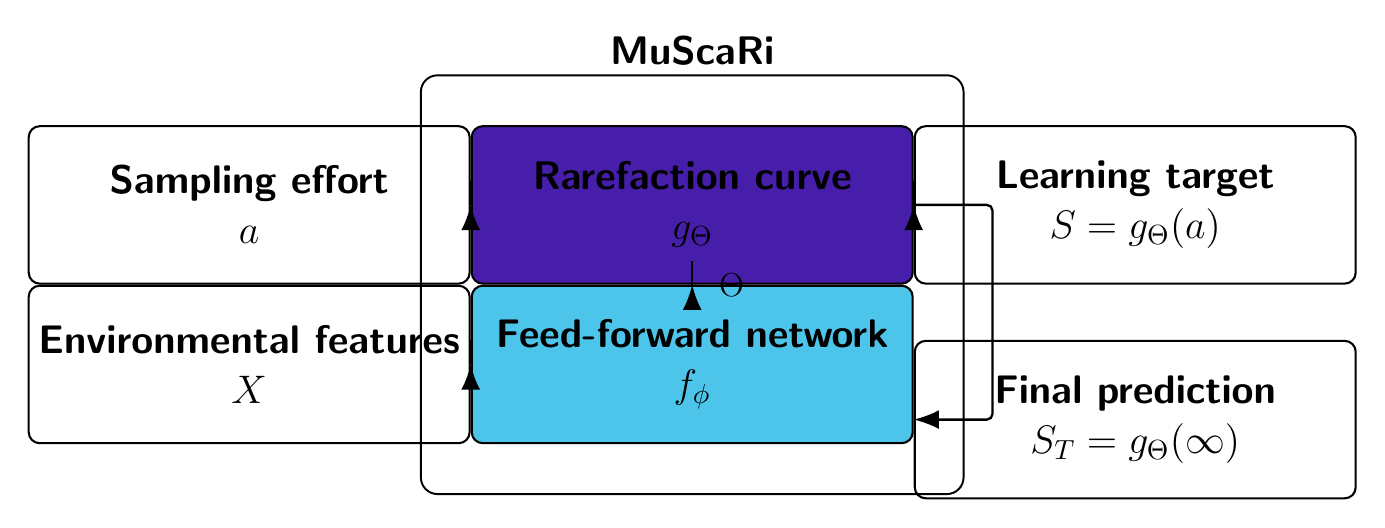
\begin{tikzpicture}[node distance=\blocksep]
      % Colors
      \definecolor{ffblue}{RGB}{77,197,235}
      \definecolor{ffpurple}{RGB}{70,30,170}
      \definecolor{ffgray}{RGB}{245,245,245}

      % Styles (modern ML-paper look)
      \tikzset{
            block/.style={draw, rounded corners=4pt, line width=0.75pt,
                                minimum height=2.0cm, minimum width=5.6cm,
                                align=center, text=black, font=\bfseries\Large},
            smallblock/.style={draw, rounded corners=4pt, line width=0.6pt,
                                       minimum height=1.1cm, minimum width=3.6cm,
                                       align=center, text=black, font=\bfseries\large},
            circleparam/.style={draw, circle, fill=white, line width=0.6pt,
                                          minimum size=0.9cm, font=\large},
            arrow/.style={-{Latex[length=3.2mm]}, line width=0.85pt, rounded corners=2pt},
            modelbox/.style={draw, rounded corners=6pt, line width=0.7pt, inner sep=18pt}
      }

      % Input features
      \node[block] (x) {Environmental features\\$X$};

      % Feed-forward network
      \node[block, fill=ffblue, right=of x] (ffn) {Feed-forward network\\$f_\phi$};

      % Rarefaction curve
      \node[block, fill=ffpurple, above=of ffn] (rare) {Rarefaction curve\\$g_\Theta$};

      % Model bounding box
      \node[modelbox, fit=(ffn)(rare), label={[font=\bfseries\Large]above:MuScaRi}] (model) {};

      % Alpha parameter (global)
      \node[block, left=of rare] (alpha) {Sampling effort\\$a$};

      % Arrows
      \draw[arrow] (x) -- (ffn);
      \draw[arrow] (ffn.north) -- (rare.south)
            node[midway, font=\large, xshift=0.5cm] (theta) {$\Theta$};
      \draw[arrow] (alpha.east) -- (rare.west);

      % Output labels
      \node[block, right=of rare] (out1)
            {Learning target\\$S=g_\Theta(a)$};
      \node[block, below=0.7cm of out1] (out2)
            {Final prediction\\$S_T=g_\Theta(\infty)$};
      \draw[arrow] (rare.east) -- (out1.west);
      \draw[arrow] (rare.east) -- ++(1.0,0) |- (out2.west);
\end{tikzpicture}
\end{document}
